\documentclass{article}

\usepackage[margin=0.85in]{geometry}
\usepackage[utf8]{inputenc}
\usepackage[T1]{fontenc}
\usepackage{url}
\usepackage{booktabs}
\usepackage{amsfonts}
\usepackage{nicefrac}
\usepackage{microtype}
\usepackage{fancyhdr}
\usepackage{graphicx}
\usepackage{amsmath}
\usepackage{amssymb}
\usepackage{algorithm}
\usepackage{algorithmic}
\usepackage{hyperref}
% Figures may sit in figures/, media/ or next to this file.
\graphicspath{{figures/}{media/}{./}}


\setlength{\headheight}{14pt}
\pagestyle{fancy}
\thispagestyle{empty}
\rhead{ \textit{ }}
\fancyhead[LO]{Reward and recipient choice}

\title{When Does Rewarding a Gift Change Whom Agents Help?}

\author{Vansh Barfiwala (24110380) \quad Pratham Choksi (24110275) \\
Shubham Chandak (24110335) \\[3pt] CS329, IIT Gandhinagar}
\begin{document}
\date{}
\maketitle

% ======================================================================

\begin{abstract}
In a spatial donation game, helping costs the donor energy while increasing the recipient's energy. Can learners sustain giving, and does rewarding marker similarity change whom they help? We train a separate PPO policy for each founder family; descendants share their family's network. Across five benefit/cost ratios, private-energy learners went extinct in every evaluation world. At ratios 4 and 6, donor-specific marker credit sustained residents in 17 of 20 seed/ratio pairs, versus zero under private reward. Equal credit for every gift also sustained all ten seeds at ratio 4. Recipient choice distinguished the incentives: marker-weighted learners directed 9.8 percentage points more gifts to qualifying recipients than a recipient-blind control. The predicted increase in marker preference with benefit/cost ratio failed, and learners continued to feed mimics. These results identify when reward shaping changes survival and targeting in this environment.
\end{abstract}

\section{Decision problem}
An agent can keep its energy while receiving gifts from others. A population can nevertheless starve if too few residents donate. Hamilton's inequality $rB>C$ motivates a test of whether the recipient matters to this decision \cite{hamilton1964}. Prior multi-agent work studies social dilemmas, gifting and intrinsic incentives \cite{leibo2017,hughes2018,jaques2019,eccles2019,lupu2020,perolat2017}. Here a learner must choose among neighbours whose observable markers and past giving can disagree.

We ask three questions. Does private-reward learning sustain cooperation already present in an untrained population? Does recipient-specific credit change the choice of recipient beyond the effect of rewarding giving in general? When a marker becomes unreliable, do learners use behavioural history instead? We also compare local and random offspring placement to test for spatial assortment. A surviving population answers the first question only in conjunction with its reward and baseline. The second requires comparing gifts among the recipients available to each donor.

\section{Implemented model and method}
\subsection{Environment}
An $18\times18$ torus holds at most 45 residents and starts with 24 founders ($E_0=30$, $E_{mitosis}=60$, $C=2$, $c_{base}=0.6$, $c_{dens}=0.08$, $\mu=0.05$, $K=10$, $b_0=0.5$, $\rho=3$). $\Omega_i$ is the set of agents within Chebyshev distance $\rho$ of $i$; it sets the density cost $c_{dens}|\Omega_i|$, and the agent observes the 8 nearest members of $\Omega_i$. Actions: stay, four moves (not giving is the ``defect'' choice) or give to one of the 8 neighbours; giving is masked unless $E_i>C$. One transition proceeds as follows: all agents act simultaneously; movement conflicts are resolved at random; donations ($-C$ to the donor, $+B$ to the recipient) and metabolic costs are applied; then every agent with $E_i\le0$ dies; only then do agents with $E_i\ge E_{mitosis}$ reproduce, if the population is below capacity and a von Neumann neighbour cell is free: the child takes the first free slot, is placed in that cell, receives half the parent's energy, a mutated chromosome and the family network, and starts with behavioural history $b_0$. Every donation creates $B-C$ net energy, so a population that does not cooperate starves. Episodes last 300 steps or until extinction. With cue noise $\nu$, every observed chromosome bit is flipped with probability $\nu$. \textbf{Mimics}: six non-donating, non-learning agents carrying the most common resident chromosome enter empty cells at step 10.

The decision process is a partially observable Markov game. Each resident observes its energy and age and, for each visible neighbour, relative position, energy, a marker cue and the fraction of recent actions spent giving. It has no direct observation of cue noise or mimic identity. The gate combines the two cues using neighbourhood context. Raw cues and the resulting affinity enter a neighbour encoder; attention combines neighbour information with the agent's own state. Five movement/stay logits and eight recipient logits form one masked categorical distribution. Gate weights alone cannot measure cue reliance because the encoder also receives the raw cues.

For resident $i$, before any split,
\[
\Delta E_i=-c_{base}-c_{dens}|\Omega_i|-C\,\mathbf{1}\{i\text{ gives}\}
+B\sum_{j\ne i}\mathbf{1}\{j\text{ gives to }i\}.
\]
Marker similarity is $h_{ij}=1-\frac18\sum_{k=1}^8|c_i^{(k)}-c_j^{(k)}|$. A newborn starts with behavioural prior $b_0$ and no past actions. Training receives the scalar reward for the chosen action. The actor does not observe the reward function, the true noise rate, or a mimic label at decision time.

\subsection{Rewards}
\label{sec:reward}
All rewards are computed before the mitosis split:
\begin{align}
\text{Energy-only (proposal):}\quad & R_i = \Delta E_i\\
\text{Inclusive fitness (Hamilton):}\quad & R_i = \Delta E_i + \textstyle\sum_{j:\,a_i=\text{give}(j)} r_{ij}\,B\\
\text{Prosocial control:}\quad & R_i = \Delta E_i + B\cdot\mathbb{I}(a_i=\text{give}(\cdot))\\
\text{Kin-blind control:}\quad & R_i = \Delta E_i + \bar r_i\, B\cdot\mathbb{I}(a_i=\text{give}(\cdot))
\end{align}
Here $r_{ij}=\min\!\big(1,\max\!\big(0,\frac{h_{ij}-\bar h}{\max(1-\bar h,\epsilon)}\big)\big)$ is computed from the \emph{true} chromosomes, with $\bar h$ the mean similarity over all distinct pairs of living residents and $\epsilon=10^{-6}$; $r_{ij}=0$ for mimics, which share no ancestry. The cue the agents observe, $\tilde r_{ij}$, uses the same formula on the observed (possibly noisy) chromosomes, with $\bar h$ taken over all distinct pairs of living agents, mimics included ($\bar h=0.5$ if fewer than two agents live). $\bar r_i$ is the mean true relatedness of the neighbours $i$ observed. The eight-bit marker measures similarity rather than pedigree ancestry. Under the inclusive reward a gift changes the donor's reward by exactly $r_{ij}B-C$, so Hamilton's rule is the immediate incentive, but the agent never sees $r_{ij}$: it must infer whom to help from the noisy cue $\tilde r_{ij}$ and behaviour $b_j$. The two controls separate \emph{kin information} from \emph{any credit for giving}: prosocial pays for every gift, and kin-blind pays the same expected kin credit whoever receives it. The inclusive-reward experiments therefore test whether learners respond to an explicitly kin-weighted incentive; they do not demonstrate spontaneous emergence of Hamilton's rule from purely individual rewards.

\subsection{Learning Algorithm}
Each of the 24 founders owns a gated-attention network (gate, neighbour encoder, 2-head attention with $d=32$, policy and value heads) and an Adam optimiser. Descendants act with their family's network, and each network is updated by PPO \cite{schulman2017} only on its own members' transitions (rollout 64, 3 epochs, minibatch 64, learning rate $3\times10^{-4}$, GAE $\lambda=0.95$, clip 0.2, entropy 0.01). Between episodes, \emph{survivor selection} draws the next founders from surviving residents, so successful lineages spread their networks (Algorithm~\ref{alg:train}). In Study C six extra slots are reserved for mimics so that every attack delivers all six. Studies B and C use $\gamma=0.9$ by default, a value selected in pilot runs; Study A and the designated sensitivity conditions use $\gamma=0.99$ (Table~\ref{tab:sens}).

\begin{algorithm}[!htbp]
\caption{Per-family PPO with inheritance and survivor selection}
\label{alg:train}
\begin{algorithmic}[1]
\STATE Create 24 founders; founder $f$ owns network $\pi_{\theta_f}$; family$(f) \leftarrow f$
\WHILE{fewer than $T$ environment steps have been collected}
    \FOR{each step of a rollout of at most 64 steps}
        \STATE Each resident $i$ samples $a_i \sim \pi_{\theta_{\mathrm{family}(i)}}(o_i)$; mimics stay
        \STATE Step the environment (one transition); compute $R_i$ (Section~\ref{sec:reward})
        \STATE Each newborn $k$ of parent $i$ inherits family$(k) \leftarrow$ family$(i)$
        \IF{no resident is left or the step count reaches 300}
            \STATE Mark the transition terminal and \textbf{break}
        \ENDIF
    \ENDFOR
    \STATE For every family $f$: PPO update of $\theta_f$ on its members' transitions only (bootstrap value 0 after a terminal step)
    \IF{the episode ended}
        \STATE Draw 24 founders with replacement from surviving residents (copy chromosome, network, optimiser); after extinction keep the networks
        \STATE Reset the environment with these founders
    \ENDIF
\ENDWHILE
\end{algorithmic}
\end{algorithm}

\subsection{Experiments, Baselines and Metrics}
We ran three studies (Table~\ref{tab:studies}). Every condition is trained independently with 10 seeds (Study A: 5) and evaluated with frozen weights in 3 fresh worlds per seed. \textbf{Baselines} run in the same worlds with the same founders: untrained networks, evolution only (selection without learning), and scripted rules: never donate, tag trust ($\tilde r>0.3$), public reputation ($b>0.5$), Tit-for-tat, and a scripted \emph{Hamilton rule using observed cues} (give to the neighbour with the highest observed $\tilde r$ if $\tilde rB>C$).

\textbf{Metrics.} \emph{Survival}: residents alive at step 300 in all 3 worlds of a seed. \emph{Donations} per resident step. \emph{Hamilton-consistent gifts}: share of gifts with $r_{ij}B>C$. \emph{Hamilton gap}: $P(\text{give}\mid\text{some neighbour has } r_{ij}B>C)-P(\text{give}\mid\text{none})$, computed within each neighbourhood size and combined with Mantel--Haenszel weights, because larger neighbourhoods offer both more give actions and more qualifying neighbours. \emph{Kin preference}: recipient's $r$ minus the neighbours' mean. \emph{Cue reliance}: per-seed conditional-logit coefficients of the chosen recipient on standardised $\tilde r$ and $b$. \emph{Mimic share}: mimics' share of post-invasion gifts. \emph{Assortment}: true-chromosome similarity of adjacent residents. \textbf{Statistics}: the training seed is the unit of inference, so the three evaluation worlds are first averaged within each seed. Means carry 95\% Student-$t$ intervals over seeds; paired contrasts use exact sign-flip tests; the ten primary contrasts (inclusive minus energy-only, on donation rate and lifetime, at each of the five $B/C$ levels) are Holm-corrected; for the two exploratory Study B survival summaries, we sum inclusive-minus-private survival differences across ratios within each seed and enumerate all $2^{10}$ sign assignments, one sign per seed. Each assignment swaps the two reward labels together at every included ratio under the sign-exchangeability null. The two overlapping summaries use the same seeds. Study C swaps labels within each seed for each reward or budget comparison; regression intervals come from a bootstrap that resamples training seeds (500 replicates).

Conditional on a donation, the fitted probability of choosing neighbour $j$ is proportional to $\exp(u_{ij})$ over the available recipients, with
\[
u_{ij}=\beta_r\tilde r_{ij}+\beta_b b_j+\beta_E E_j+\beta_{rB}\tilde r_{ij}(B/C).
\]
Our directional prediction was $\beta_{rB}>0$. This coefficient describes changes in recipient preference among observed gifts. Prosocial populations can survive with little selectivity, and an extinct population supplies no late recipient choices. The choice model uses a seed bootstrap within each ratio; the joint survival test above instead keeps a seed together across ratios.

\begin{table}[!htbp]
\centering
\caption{Studies (all trained models and evaluation logs are public).}
\label{tab:studies}
\small
\begin{tabular}{p{0.065\textwidth}p{0.26\textwidth}p{0.58\textwidth}}
\toprule
\textbf{Study} & \textbf{Setup} & \textbf{Conditions} \\
\midrule
A & Energy-only reward, 2{,}048 steps, 5 seeds & 19 robustness conditions (gate, MLP, noise, mimics, $B/C$, mutation, placement, selection, learning rate, entropy, $4\times$ training) \\
B & 8{,}192 steps, 10 seeds, 200 models & Energy-only vs inclusive at $B/C\in\{1,1.5,2.5,4,6\}$; noise, mimics, gate, MLP, placement, $\gamma=0.99$ \\
C & $B/C=4$, 10 seeds, 180 models & Prosocial and kin-blind controls, noise, mimics, gate, MLP, mutation, $\gamma=0.99$ for both rewards, $4\times$ training \\
\bottomrule
\end{tabular}
\end{table}

% ======================================================================
\section{Results}
% ======================================================================

\subsection{Private reward, shaped reward and population survival}
With the energy-only reward, \textbf{all 90 of 90} learning runs of Study A gave less than untrained networks with the same founders, whatever the architecture, noise, mutation, selection or training length. Study B (Table~\ref{tab:main}, Fig.~\ref{fig:sweep}) shows why this matters: energy-only populations die at every $B/C$ (0/50), even where untrained networks survive. Adding the kin term keeps populations alive: 18/50 versus 0/50 overall (36 percentage points) and \textbf{17/20 versus 0/20 at $B/C\ge4$} (85 percentage points). All ten seed blocks favoured the shaped reward in each summary; each exact two-sided $p=2/1024=0.00195$. Inclusive learners gave more than energy-only learners in all 10 seeds at every $B/C\ge1.5$ (Holm $p=0.02$).

\begin{table}[!htbp]
\centering
\caption{Study B: seeds surviving all evaluation worlds and donations per resident step (mean [95\% CI], 10 seeds).}
\label{tab:main}
\small
\begin{tabular}{c ccc ccc}
\toprule
 & \multicolumn{3}{c}{\textbf{Seeds surviving}} & \multicolumn{3}{c}{\textbf{Donations / resident step}} \\
\cmidrule(lr){2-4}\cmidrule(lr){5-7}
$B/C$ & Inclusive & Energy & Untrained & Inclusive & Energy-only & Untrained \\
\midrule
1.0 & 0/10 & 0/10 & 0/10 & 0.009 [0.006, 0.011] & 0.006 [0.005, 0.007] & 0.322 \\
1.5 & 0/10 & 0/10 & 0/10 & 0.011 [0.009, 0.013] & 0.007 [0.006, 0.008] & 0.316 \\
2.5 & 1/10 & 0/10 & 10/10 & 0.242 [0.078, 0.406] & 0.005 [0.003, 0.007] & 0.498 \\
4.0 & \textbf{7/10} & 0/10 & 10/10 & 0.405 [0.180, 0.629] & 0.016 [0.007, 0.026] & 0.568 \\
6.0 & \textbf{10/10} & 0/10 & 10/10 & \textbf{0.803} [0.686, 0.920] & 0.032 [0.018, 0.046] & 0.515 \\
\bottomrule
\end{tabular}
\end{table}

\begin{figure}[!htbp]
\centering
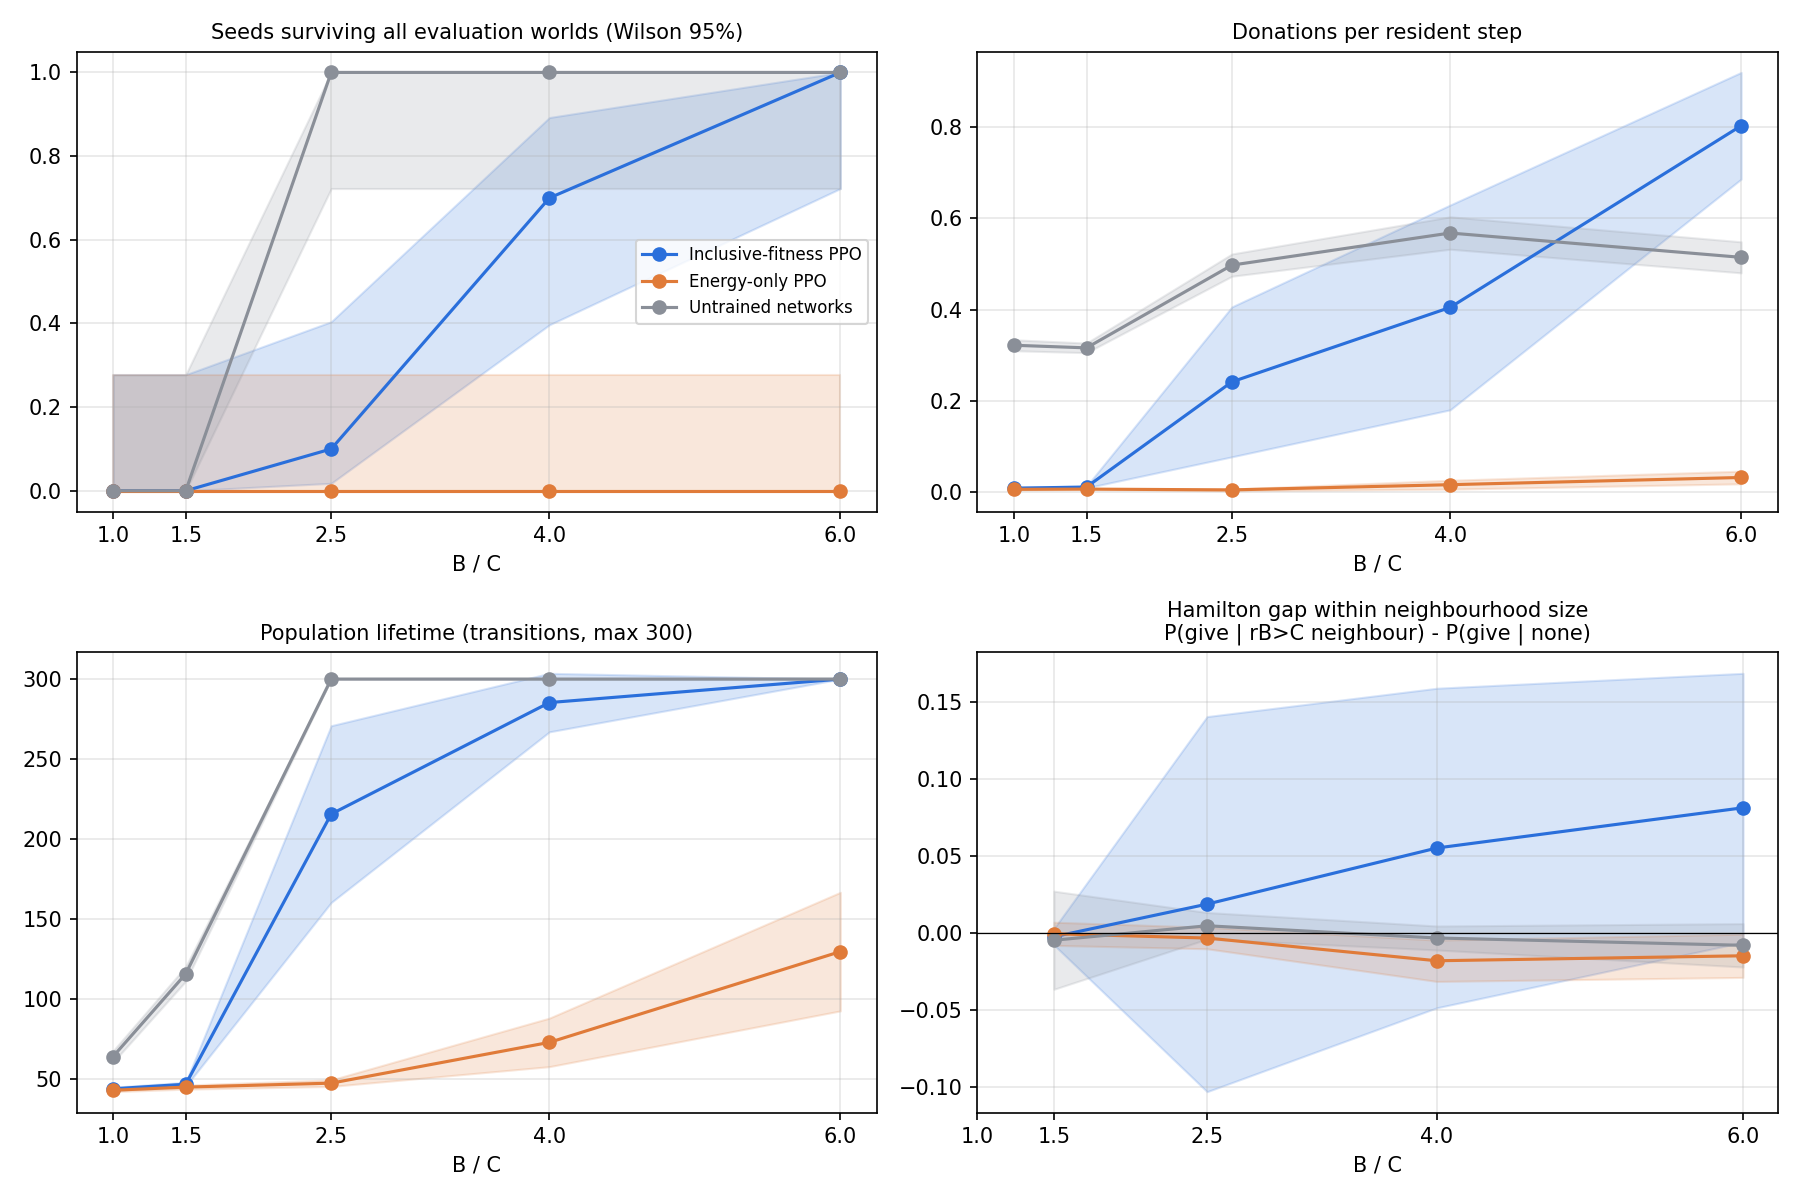
\includegraphics[width=0.72\textwidth]{bc_sweep.png}
\caption{Study B across $B/C$ (10 seeds, 95\% intervals): survival, donations, lifetime and Hamilton gap. Inclusive PPO (blue), energy-only PPO (orange), untrained networks (grey).}
\label{fig:sweep}
\end{figure}

\textbf{Mechanism.} Energy-only populations die out \emph{during} training (Fig.~\ref{fig:curves}): every gift is an immediate loss of $C$ to the donor, and the donor's reward contains no credit for the recipient's gain. Our hypothesis, not directly tested, is that each family's gradient removes giving faster than survivor selection can favour givers.

\begin{figure}[!htbp]
\centering
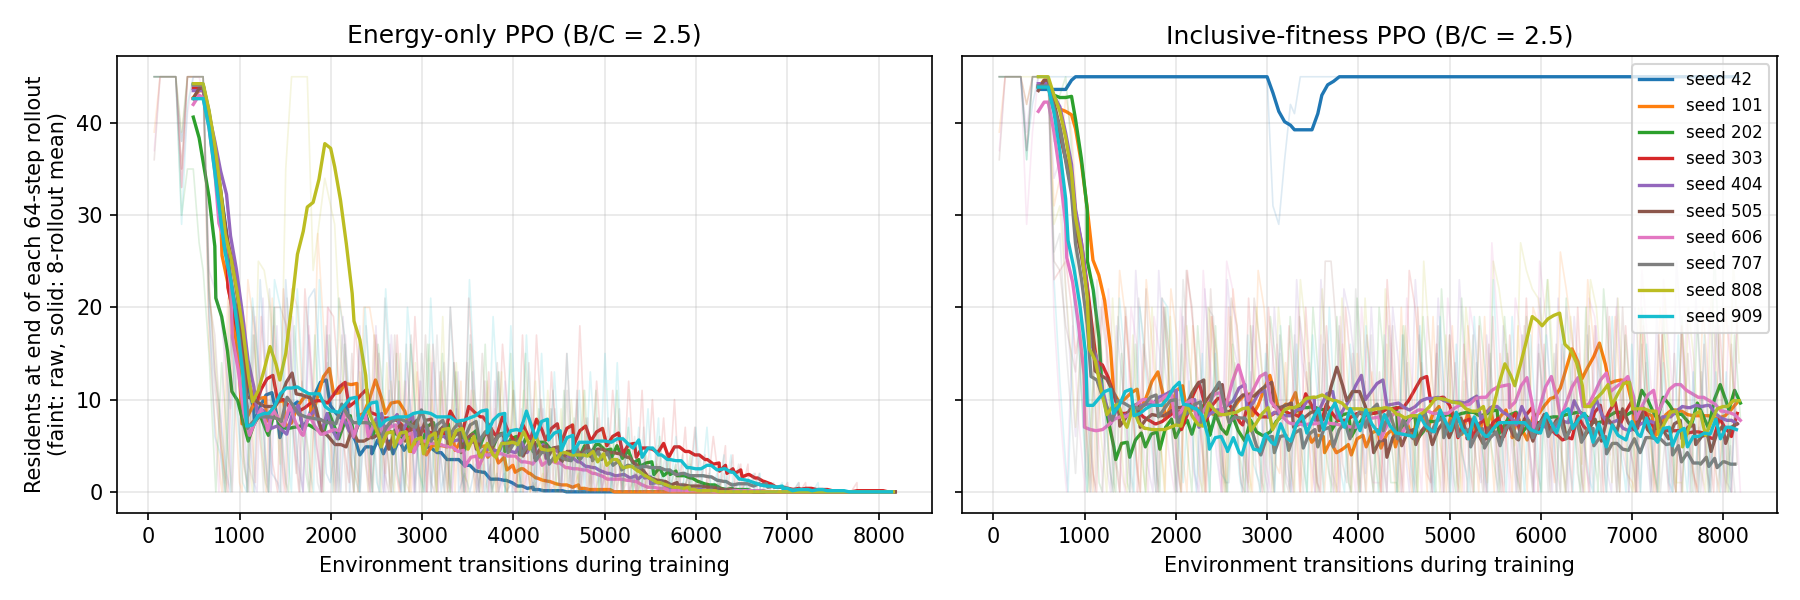
\includegraphics[width=0.85\textwidth]{learning_curves.png}
\caption{Residents during training at $B/C=2.5$ (one line per seed): energy-only populations go extinct; under the inclusive reward one seed stays at capacity and the others persist at small sizes.}
\label{fig:curves}
\end{figure}

\subsection{Does recipient choice track the Hamilton threshold?}
Under the inclusive reward, learned donation rates were low at the two lowest tested ratios: $B/C=1$ makes $rB>C$ impossible ($r>1$), whereas $B/C=1.5$ requires $r>2/3$. At $B/C=6$ inclusive learners gave more than untrained networks (9/10 seeds). The scripted Hamilton rule using observed cues switches on at a similar point (Fig.~\ref{fig:strat}). Learners choose more related recipients (conditional-logit coefficient 1.72 [0.78, 2.66]); the predicted increase of this effect with $B/C$ was not found ($-0.26$ [$-0.42$, $-0.10$]). One reading is a threshold policy that discriminates less once most neighbours qualify; this is a post-hoc interpretation, not confirmation of the predicted interaction.

\begin{figure}[!htbp]
\centering
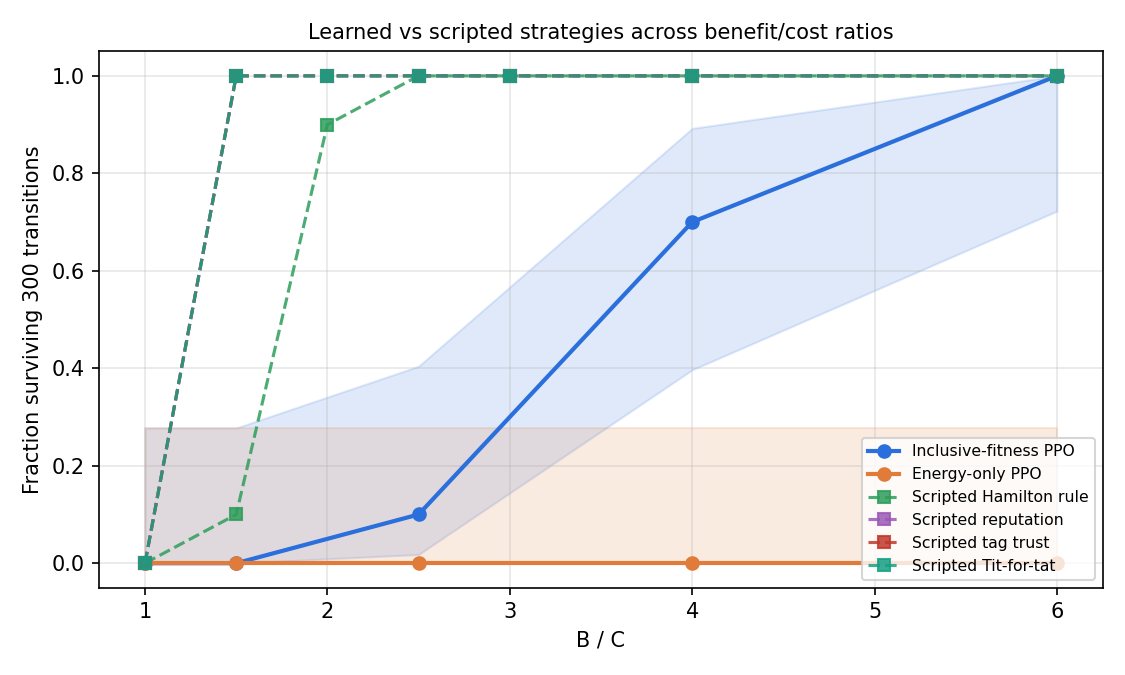
\includegraphics[width=0.58\textwidth]{strategies_vs_bc.png}
\caption{Survival across $B/C$: learned rewards (10 seeds) and scripted strategies (10 worlds each).}
\label{fig:strat}
\end{figure}

\subsection{Kin-Weighted Rewards Improve Targeting}
Paying for every gift (prosocial) kept all populations alive (Table~\ref{tab:controls}); no significant survival difference was detected between the inclusive reward and either control. The kin-weighted reward improved \emph{targeting}: compared with the kin-blind reward of the same expected size, inclusive learners give more gifts to recipients with $rB>C$ (+0.098, 8/10 seeds, $p=0.010$), prefer more related recipients ($p=0.025$) and rely more on the genetic cue ($p=0.016$; against prosocial $p=0.004$).

\begin{table}[!htbp]
\centering
\caption{Study C: reward controls at $B/C=4$ (10 seeds; mean [95\% CI]). Intervals are unconstrained Student-$t$ intervals over seeds, so a bound can pass a metric's range (e.g.\ 1.001 for a donation rate near its maximum of 1).}
\label{tab:controls}
\small
\resizebox{\textwidth}{!}{
\begin{tabular}{lccccc}
\toprule
\textbf{Reward} & \textbf{Survive} & \textbf{Donations/step} & \textbf{Gifts with $rB>C$} & \textbf{Kin preference} & \textbf{Genetic share of choice} \\
\midrule
Inclusive ($r_{ij}B$) & 7/10 & 0.405 [0.180, 0.629] & 0.499 [0.406, 0.592] & 0.039 [0.001, 0.078] & 0.780 [0.657, 0.904] \\
Kin-blind ($\bar r_i B$) & 6/10 & 0.307 [0.085, 0.529] & 0.401 [0.327, 0.475] & 0.001 [$-$0.007, 0.010] & 0.444 [0.284, 0.604] \\
Prosocial ($B$ per gift) & 10/10 & 0.994 [0.988, 1.001] & 0.487 [0.442, 0.532] & 0.009 [0.002, 0.015] & 0.363 [0.166, 0.560] \\
Energy-only & 0/10 & 0.016 [0.007, 0.026] & 0.205 [0.101, 0.309] & $-$0.042 [$-$0.081, $-$0.003] & -- \\
\bottomrule
\end{tabular}}
\end{table}

\subsection{Cue corruption and genetic mimicry}
Corrupting the genetic cue reduced its measured influence on recipient choice (Fig.~\ref{fig:cue}a; noise 0 vs 0.5: +0.217, 8/10 seeds, $p=0.014$; lower genetic share at noise 0.25 in all 10 seeds, $p=0.002$), which supports reduced genetic-cue reliance, but not the proposed shift toward behavioural history or resistance to mimicry. Agents did \emph{not} shift to behavioural history: its coefficient stayed near zero, and survival fell from 7/10 to 2/10. No learner avoided mimics (Fig.~\ref{fig:cue}b): inclusive learners gave them 17\% of gifts, about what untrained networks give (13\%), while a one-line public-reputation rule gives them nothing because a mimic's giving record is zero. No significant advantage of the learned gate over a fixed gate was detected ($p=0.44$).

\begin{figure}[!htbp]
\centering
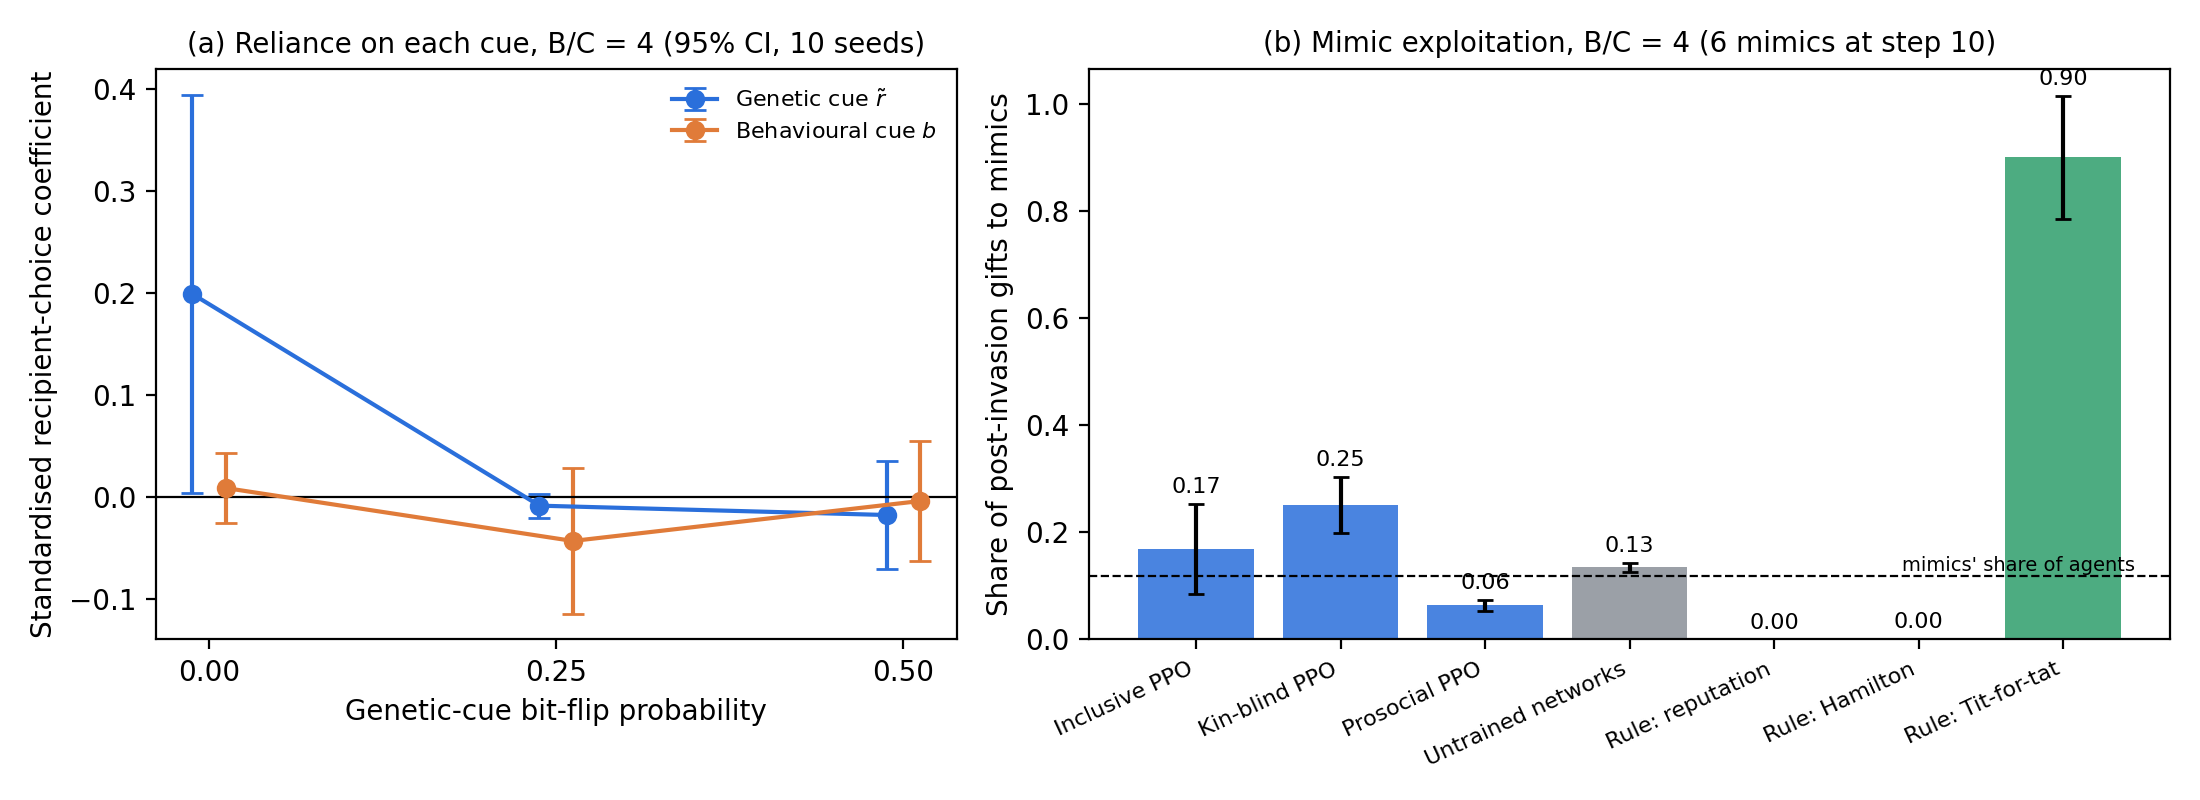
\includegraphics[width=0.92\textwidth]{cue_and_mimics.png}
\caption{(a) Recipient-choice coefficients of the genetic and behavioural cues as the genetic cue is corrupted ($B/C=4$). (b) Share of post-invasion gifts to mimics; dashed line: mimics' share of agents.}
\label{fig:cue}
\end{figure}

\subsection{Spatial assortment and sensitivity}
\begin{table}[!htbp]
\centering
\caption{Assortment, sensitivity and ablations (10 seeds each).}
\label{tab:sens}
\small
\begin{tabular}{p{0.26\textwidth}p{0.37\textwidth}p{0.29\textwidth}}
\toprule
\textbf{Check} & \textbf{Result} & \textbf{Reading} \\
\midrule
Local vs random offspring placement & adjacent similarity $+0.083$ ($p=0.31$, $B/C=2.5$); $-0.015$ ($p=0.78$, $B/C=4$) & No significant assortment difference detected \\
$\gamma=0.99$ for both rewards, $B/C=4$ & survival 2/10 vs 2/10 (paired $p=1.0$) & Survival advantage absent at the tested $\gamma=0.99$ \\
$4\times$ training, $B/C=2.5$ & survival 2/10 vs 1/10 & No improvement detected with $4\times$ training \\
Evolution only (no learning), $B/C=4$ & 10/10 survive; learning targets kin better (+0.147, $p=0.006$) & Selection keeps giving; learning improves targeting \\
Attention vs MLP, $B/C=4$ & gifts with $rB>C$ $+0.129$ ($p=0.016$) & Attention improved kin targeting here \\
Mutation 0.20 vs 0.05 & donations $-0.244$ ($p=0.014$), survival 4/10 & Higher mutation reduced cooperation in this condition \\
\bottomrule
\end{tabular}
\end{table}

No significant assortment difference was detected (Table~\ref{tab:sens}); a possible explanation is that survivor selection makes populations near-clonal, so neighbours are related wherever offspring are placed.

\textbf{Discussion and limitations.} At fixed architecture, changing the reward changed both the amount of giving and survival at the higher ratios. These experiments show that learners respond to a kin-weighted incentive; they do not show Hamilton's rule emerging spontaneously from purely individual rewards. Kin recognition is the weak link: learners mainly learn \emph{whether} to give rather than \emph{to whom}, did not learn to use behaviour, and kept feeding mimics. Limitations: the inclusive reward uses true relatedness, which real organisms do not observe; the survival advantage was absent at the tested $\gamma=0.99$; ten seeds and 8{,}192 steps per run limit power; mimics are scripted; one environment family is tested.

% ======================================================================
\section{Conclusion}
% ======================================================================
Under the tested private reward, PPO reduced giving below the untrained baseline. At $B/C=4$, equal credit for every gift sustained 10/10 seeds, recipient-specific credit sustained 7/10, and private credit sustained 0/10. Survival therefore cannot identify marker discrimination. The matched kin-blind control provides the evidence for targeting: rewarding the actual recipient's marker increased the share of qualifying gifts. The predicted positive cue-by-ratio interaction failed and the survival advantage disappeared at the tested discount of 0.99. A useful next test would hold the incentive fixed and change only which recipient cues the learner can observe.

% ======================================================================
\section{Contribution}
% ======================================================================
\begin{itemize}
    \item \textbf{Vansh Barfiwala:} Spatial Donation Game environment: energy dynamics, metabolic and density costs, starvation and mitosis, the corrected agent-pooling algorithm with capacity tracking and the mimic slot reserve, and the environment tests. Final revision: paired survival analysis, verification against evaluation logs, and alignment of the proposal, report and project page.
    \item \textbf{Pratham Choksi:} Gated-attention policy: contextual gating network ($w^g, w^b$) with neighbourhood statistics, baseline-corrected relatedness $\tilde r_{ij}$, cue noise and mimics, the joint masked action distribution, and the gate, attention and MLP ablations.
    \item \textbf{Shubham Chandak:} Per-family PPO training with inheritance and survivor selection, the reward variants (inclusive, prosocial, kin-blind), the experiment pipeline for Studies A--C, statistical analysis (sign-flip tests, conditional logit, Hamilton gap, assortment), the verification script and the interactive project page.
\end{itemize}

\textbf{Reproducibility.} The sampled Python trajectories depend on library versions. Use Python 3.12, PyTorch 2.5.1 and NumPy 2.3.2 for exact replay; the saved world logs also support independent statistical checks. The project page \url{https://chandak-shubham.github.io/cs329_project/} runs the committed trained models in the browser: choose one of the supported training conditions (16 conditions of Studies B and C, 10 seeds each), watch the population, add mimics or change $B$ and $C$, and press \emph{Reproduce a result} to rerun all 10 seeds and compare them with the recorded Python evaluation. Its research section, all figures, tables (\texttt{results/}) and the 475 trained models (\texttt{models/}) are in the repository \url{https://github.com/chandak-Shubham/cs329_project}, together with \path{evaluation/verify_hamilton.py}, which verifies the integrity (SHA-256 and training settings) of every Study B and C checkpoint and replays selected checkpoints exactly by default, or all of them with \texttt{--all}.

\begin{thebibliography}{99}
\bibitem{veritasium2025} Muller, D. [Veritasium]. (2025). \textit{The Most Controversial Idea In Biology}. YouTube.
\bibitem{hamilton1964} Hamilton, W. D. (1964). \textit{The genetical evolution of social behaviour. I \& II}. J. Theor. Biol., 7(1), 1-52.
\bibitem{dawkins1976} Dawkins, R. (1976). \textit{The Selfish Gene}. Oxford University Press.
\bibitem{leibo2017} Leibo, J. Z., et al. (2017). \textit{Multi-agent reinforcement learning in sequential social dilemmas}. AAMAS.
\bibitem{hughes2018} Hughes, E., et al. (2018). \textit{Inequity aversion improves cooperation in intertemporal social dilemmas}. NeurIPS.
\bibitem{jaques2019} Jaques, N., et al. (2019). \textit{Social influence as intrinsic motivation for multi-agent deep RL}. ICML.
\bibitem{eccles2019} Eccles, T., et al. (2019). \textit{Learning reciprocity in complex sequential social dilemmas}. arXiv:1903.08082.
\bibitem{lupu2020} Lupu, A., \& Precup, D. (2020). \textit{Gifting in multi-agent reinforcement learning}. AAMAS.
\bibitem{perolat2017} Perolat, J., et al. (2017). \textit{A multi-agent RL model of common-pool resource appropriation}. NeurIPS.
\bibitem{schulman2017} Schulman, J., et al. (2017). \textit{Proximal policy optimization algorithms}. arXiv:1707.06347.
\end{thebibliography}

\end{document}
